\subsection{L'équipe Avalon en détails}
L'équipe dont je fais partit durant ce stage est l'équipe Avalon. Cette équipe créée le 1er Février 2012 \cite{avalonAR2012} est une équipe-projet du Laboratoire de l'Informatique du Parallélisme commune à l'\gls{inria} composée de 22 membres : 8 universitaires permanents, 2 universitaires temporaires, 4 membres permanents et 8 doctorants. Elle est située au troisième étage de l'aile sud du bâtiment M7 sur le site Monod de l'École Normale Supérieure de Lyon.

\subsubsection{Les membres de l'équipe}
Parmi les 22 membres de l'équipe, voici un rapide aperçu de ceux que j'ai côtoyé durant mon stage :\\

\textbf{Universitaires permanents}
\begin{figure}[h!]
   \begin{minipage}{0.33\textwidth}
		\centering
		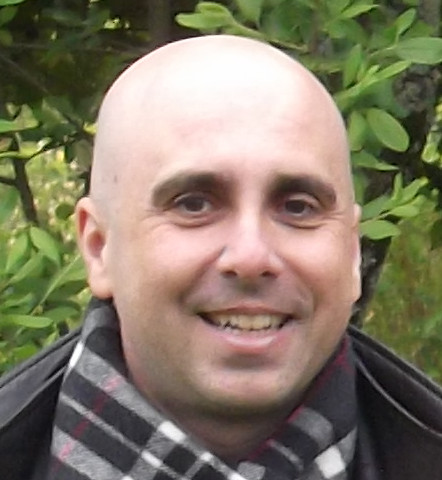
\includegraphics[height=3cm]{partie1/images/christian.jpg}\\
		\textbf{Christian Perez}\\
		Chef de l'équipe\\Chercheur sénior Inria
	\end{minipage}\hfill
	\begin{minipage}{0.33\textwidth}
		\centering
		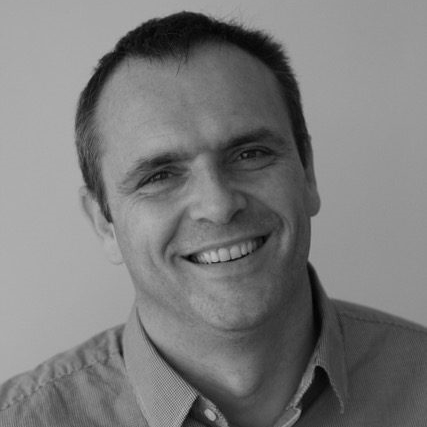
\includegraphics[width=3cm]{partie1/images/eddy.jpeg}\\
		\textbf{Eddy Carron}\\
		Responsable administratif\\Enseignant chercheur
	\end{minipage}\hfill
	\begin{minipage}{0.33\textwidth}
		\centering
		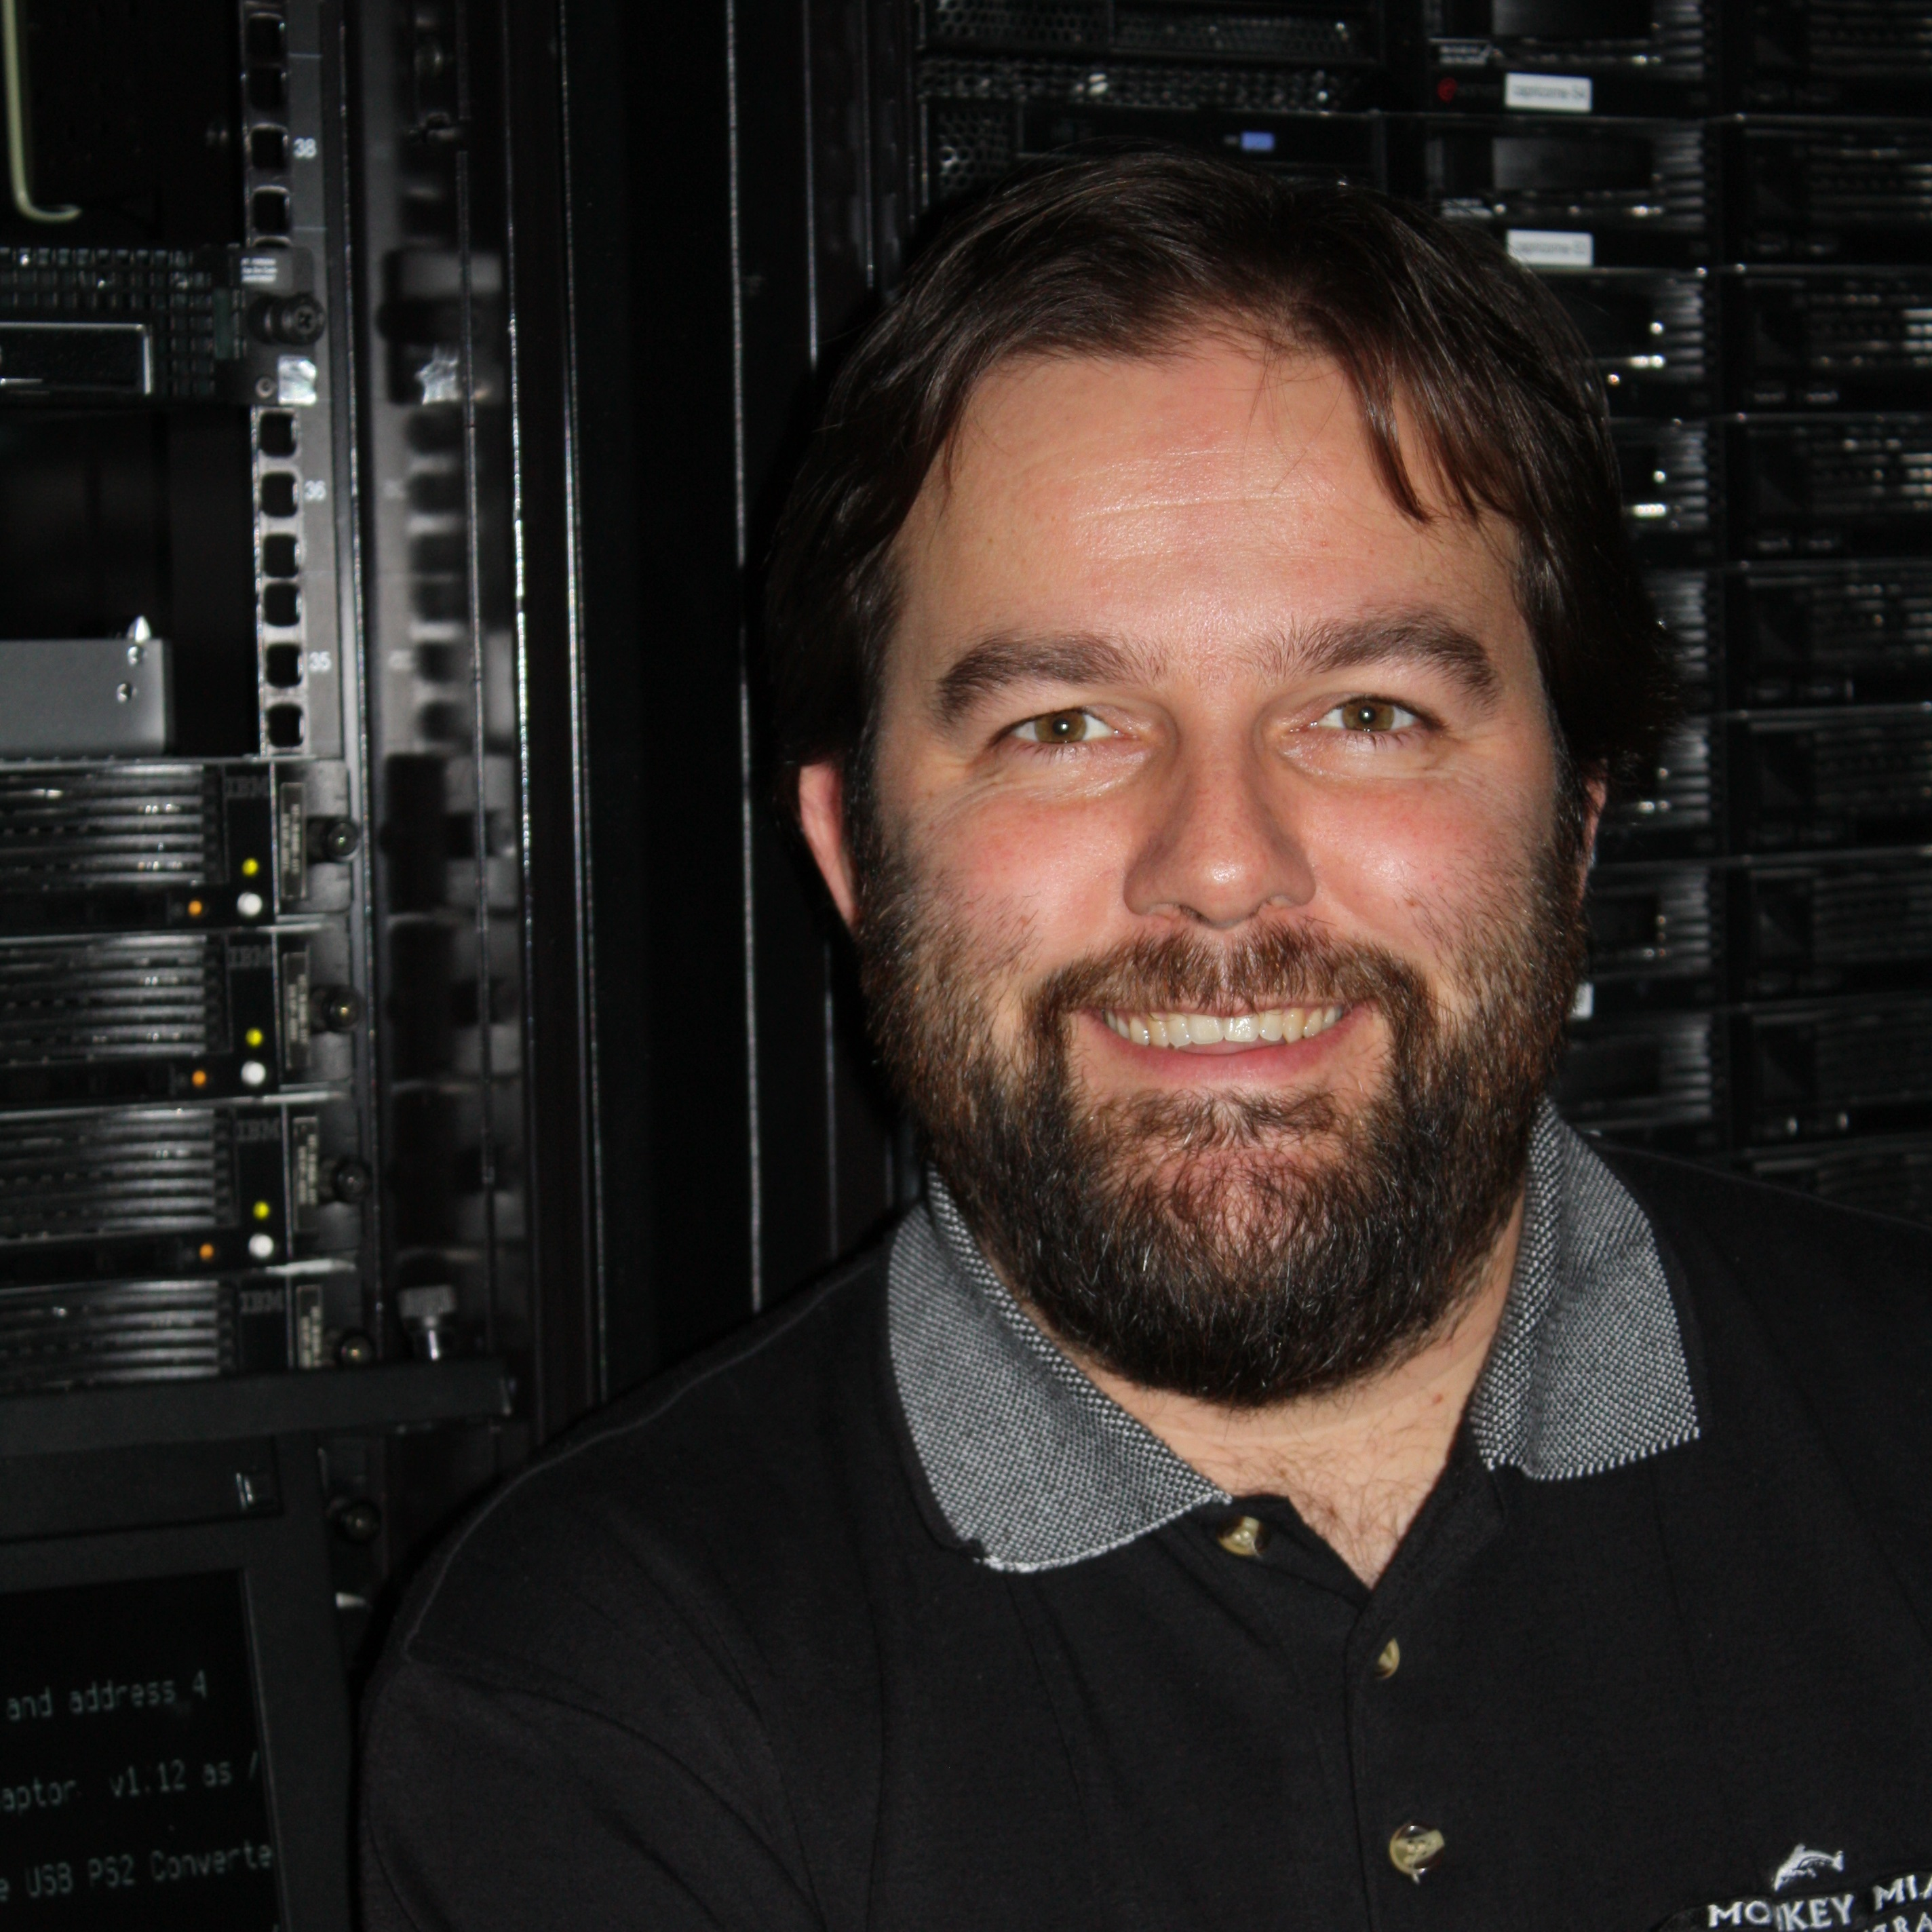
\includegraphics[width=3cm]{partie1/images/laurent.jpg}\\
		\textbf{Laurent Lefèvre}\\
		Mon maître de stage\\Chercheur Inria
	\end{minipage}
\end{figure}

\textbf{Universitaires temporaires}
\begin{figure}[h!]
	\begin{minipage}{0.48\textwidth}
		\centering
		
\includegraphics[height=3cm]{partie1/images/marco.jpg}\\
		\textbf{Marcos Dias de Assuncao}\\
		Chercheur
	\end{minipage}\hfill
	\begin{minipage}{0.48\textwidth}
		\centering
		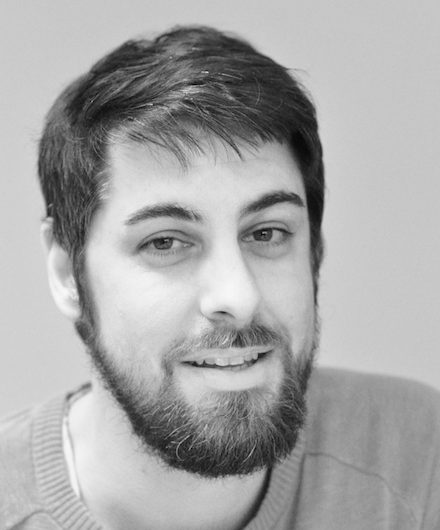
\includegraphics[height=3cm]{partie1/images/cyril.jpg}\\
		\textbf{Cyril Seguin}\\
		Chercheur PostDoc\\Expert Cloud et Sécurité
	\end{minipage}\hfill
\end{figure}

\textbf{Équipe}
\begin{figure}[h!]
	\begin{minipage}{0.33\textwidth}
		\centering
		
\includegraphics[height=3cm]{partie1/images/evelyne.jpeg}\\
		\textbf{Evelyne Blesle}\\
		Assistante administrative
	\end{minipage}\hfill
	\begin{minipage}{0.33\textwidth}
		\centering
		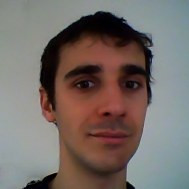
\includegraphics[width=3cm]{partie1/images/simon.jpeg}\\
		\textbf{Simon Delamare}\\
		Ingénieur de recherche
	\end{minipage}\hfill
	\begin{minipage}{0.33\textwidth}
		\centering
		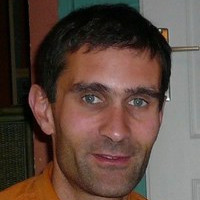
\includegraphics[width=3cm]{partie1/images/matthieu.jpeg}\\
		\textbf{Matthieu Imbert}\\
		Ingénieur de recherche
	\end{minipage}
\end{figure}
\newpage
\textbf{Doctorants}
\begin{figure}[h!]
	\begin{minipage}{0.33\textwidth}
		\centering
		
\includegraphics[height=3cm]{partie1/images/issam.jpeg}\\
		\textbf{Issam Raïs}\\
		Thèse sur l'étude de la consommation énergétique des supercalculateurs
	\end{minipage}\hfill
	\begin{minipage}{0.33\textwidth}
		\centering
		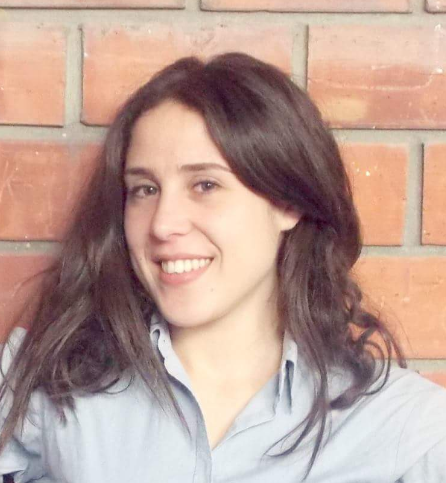
\includegraphics[width=3cm]{partie1/images/dorra.png}\\
		\textbf{Dorra Boughzala}\\
		Thèse sur la simulation de la consommation d'énergie des architecture hétérogènes
	\end{minipage}\hfill
	\begin{minipage}{0.33\textwidth}
		\centering
		
\includegraphics[width=3cm]{partie1/images/alexandre.jpg}\\
		\textbf{Alexandre da Silva Veith}\\
		Thèse sur les algorithmes pour l'analyse des flux élastiques du Big-Data
	\end{minipage}
\end{figure}
\begin{figure}[h!]
	\begin{minipage}{0.33\textwidth}
		\centering
		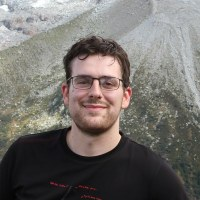
\includegraphics[height=3cm]{partie1/images/hadrien.jpeg}\\
		\textbf{Hadrien Croubois}\\
		Spécialisé dans les processus parallèles et les systèmes distribués
	\end{minipage}\hfill
	\begin{minipage}{0.33\textwidth}
		\centering
		
\includegraphics[width=3cm]{partie1/images/felipe.jpg}\\
		\textbf{Felipe Rodrigo de Souza}\\
		Thèse sur les algorithmes de provisionnement des réseaux
	\end{minipage}\hfill
	\begin{minipage}{0.33\textwidth}
		\centering
		
\includegraphics[width=3cm]{partie1/images/valentin.jpg}\\
		\textbf{Valentin Lorentz}\\
		Thèse sur la traçabilité énergétique des données
	\end{minipage}
\end{figure}

\subsubsection{Le contexte de création}
Formée le 1 Février 2012, l'équipe Avalon est une véritable réponse aux changements effrénés de l'informatique.
L'évolution très rapide du matériel informatique en terme de communication, de traitement de données et de virtualisation à fait émerger des nouveaux besoins pour l'utilisateur. En effet la complexité des systèmes informatiques augmente !
Il existe aujourd'hui de nombreuses variétés de plateformes à grande échelles disponibles pour des chercheurs ou des industriels qui souhaitent satisfaire leurs besoins en traitement de données : agrégation de \glspl{cluster}, grand \glspl{datacenter}, supercalculateurs etc.
Chacune de ces plateforme disposent de spécificités intrinsèques, d'accès et d'utilisation qui ont un impact important sur l'architecture et l'exécution des applications qui souhaitent les utiliser.
Elles intègrent de nombreuses fonctionnalités obligatoires comme le sécurité, la virtualisation, le \gls{load-balancing} ou autres qui augmentent encore plus leur complexité d'utilisation.
C'est dans ce contexte que l'équipe Avalon a été créée, la réponse qu'elle apporte est d'aller plus loin dans l'abstraction de ces plateformes pour assurer à l'utilisateur une utilisation simplifiée tout en gardant l'ensemble des fonctionnalités disponibles. \cite{avalonAR2012}

\subsubsection{La vision de l'équipe}
La vision de l'équipe Avalon est de considérer l'ensemble du système, de la ressource à l'application, afin de concevoir des outils simples à utiliser par les programmeurs tout en permettant une exploitation efficace des ressources.
L'équipe se concentre en particulier sur la gestion de l'élasticité (i.e\ la capacité à s'adapter aux besoins des applications le plus rapidement possible) des plateforme parallèles et distribués ainsi que leur efficacité énergétique. \cite{avalonAR2012}\\

L'équipe souhaite pouvoir mettre à disposition d'autres équipes de recherche travaillant dans d'autres sciences des ressources informatiques à haute performance de manière simple à utiliser.

Voici quelques exemples de disciplines qui pourrait avoir recours aux travaux de l'équipe Avalon :
\begin{itemize}
	\item La biologie, avec par exemple le séquençage de l'ADN,
	\item L'étude du climat, qui demande une quantité de paramètres impressionnante pour simuler les changements de climat prochains,
	\item L'astrophysique, qui est demandeuse de simulations pour comprendre les phénomènes physique qui nous entoure, la formation des galaxies, pour étudier la matière noire etc.
\end{itemize}